
%(BEGIN_QUESTION)
% Copyright 2010, Tony R. Kuphaldt, released under the Creative Commons Attribution License (v 1.0)
% This means you may do almost anything with this work of mine, so long as you give me proper credit

This fluid diagram shows the components and connections of a Bettis self-contained hydraulic module used to automatically shut off a ``line valve'' on a natural gas pipeline in the event of the pipeline pressure going outside of its limits (either falling below the low-pressure limit or rising above the high-pressure limit):

$$\includegraphics[width=15.5cm]{i02519x01.eps}$$

Suppose this line valve automatically trips because the gas compressor feeding the line with pressure happens to shut down one day.  Examine this diagram, and from it determine what steps a technician would need to go through in order to get the line valve open again.  Be sure to make note of pressure gauge readings in your re-set procedure!

\underbar{file i02519}
%(END_QUESTION)





%(BEGIN_ANSWER)

Make sure the Auto/Manual valve is in the ``Auto'' position, the solenoid valve is not tripped, and hold in the ``Reset'' valve lever while pumping the hand pump lever back and forth.  Both the HP and LP gauges should begin to rise.  The LP gauge will stabilize at its setpoint before the HP gauge stabilizes at its setpoint.  When you reach a point where neither gauge pressure rises despite continued pumping, you may stop pumping and release the ``Reset'' valve lever.

%(END_ANSWER)





%(BEGIN_NOTES)


%INDEX% Final Control Elements, valve: fail-safe solenoids

%(END_NOTES)


